\documentclass{article}
% \documentclass[twocolumn]{article}
\usepackage{graphicx} % Required for inserting images
\usepackage{tikz} 
\usepackage{amsmath}
\usepackage{booktabs}
\usepackage{multirow}
\usepackage{tabularx}
\usepackage{array}

\newcommand{\mybox}[5]{
    \begin{center}
    \begin{tikzpicture}
        \node[anchor=text,text width=\columnwidth+1.0cm, draw, rounded corners, line width=1pt, fill=#3, inner sep=5mm] (big) {\\#4};
        \node[draw, rounded corners, line width=.5pt, fill=#2, anchor=west, xshift=5mm] (small) at (big.north west) {#1};
    \end{tikzpicture}
    % \caption{#5}
    \end{center}
}


\title{25.9.30 halo2-lib and Midnight-zk}

\author{Wuyunsiqin \quad \quad Bingsheng Zhang \\ 
Zhejiang University, CHN \\
22521299@zju.edu.cn \quad bingsheng@zju.edu.cn}
% \date{May 20 2025}




\begin{document}

\maketitle


\section{Comparison between halo2-lib and Midnight zk}

\subsection{Protocol Stack Differences}

\texttt{halo2-lib} is Axiom's set of halo2 extensions geared toward flexible gadget development, while Midnight zk packages the proving stack that powers Midnight's privacy chain. The two ecosystems diverge in several foundational aspects:

\begin{itemize}
    \item \textbf{Curves and fields.} \texttt{halo2-lib} ships turn-key support for multiple curves (BN254, secp256k1 and Grumpkin via the \texttt{halo2-ecc} crate) on top of the generic halo2 curve abstractions. Midnight zk narrows the focus to the BLS12-381 pairing curve and its embedded Jubjub subgroup, matching the primitives used by the Midnight protocol.
    \item \textbf{Polynomial commitments and SRS tooling.} Both stacks rely on the PLONK proving system with KZG commitments, but their SRS workflows differ. \texttt{halo2-lib} expects the caller to provision halo2's \texttt{Params} (often generated for BN254) and exposes low-level access to the underlying commitments. Midnight zk integrates a dedicated \texttt{proof-system} crate that manages SRS down-sizing, proving/verification key material, and proof aggregation tailored to its BLS12-381 setup.
    \item \textbf{Circuit builder philosophy.} \texttt{halo2-lib}'s \texttt{halo2-base} builder emphasises dynamic gate composition—developers control advice/fixed column counts per circuit to optimise cost. Midnight zk's \texttt{ZkStdLib} instead advertises a declarative architecture switch (enabling Jubjub, Poseidon, SHA-256, etc.) so relation authors focus on high-level constraints while the library configures chips consistently across proofs.
    \item \textbf{Gadget catalogue and interoperability.} \texttt{halo2-lib} targets Ethereum-centric use cases (Poseidon with adjustable rate, Keccak/SHA-256, big-integer arithmetic, pairing gadgets) and interoperates with the wider halo2 community crates. Midnight zk aligns its gadget set with Midnight's application layer (Jubjub MSM, recursive proof verification, variable-length data parsing) and keeps API versions in lockstep with the Midnight aggregator.
\end{itemize}

\begin{table}[htbp]
    \centering
    \caption{Architectural comparison between \texttt{halo2-lib} and Midnight zk.}
    \label{tab:lib-architecture}
    \begingroup
    \renewcommand{\arraystretch}{1.2}
    \begin{tabularx}{\textwidth}{>{\raggedright\arraybackslash}p{3.0cm} >{\raggedright\arraybackslash}X >{\raggedright\arraybackslash}X}
        \toprule
        Aspect & \texttt{halo2-lib} & Midnight zk \\
        \midrule
        Curve support & BN254, secp256k1, Grumpkin, etc. & BLS12-381 pairing curve with embedded Jubjub subgroup \\
        Circuit configuration & \texttt{halo2-base} gate builder with tunable advice/fixed columns & Declarative \texttt{ZkStdLib} architecture toggles enabled chips consistently \\
        Integration targets & Broad halo2 ecosystem and third-party zk applications & Midnight ledger stack and associated aggregator tooling \\
        \bottomrule
    \end{tabularx}
    \endgroup
\end{table}

\subsection{System Configuration}

\begin{figure}[htbp]
    \centering
    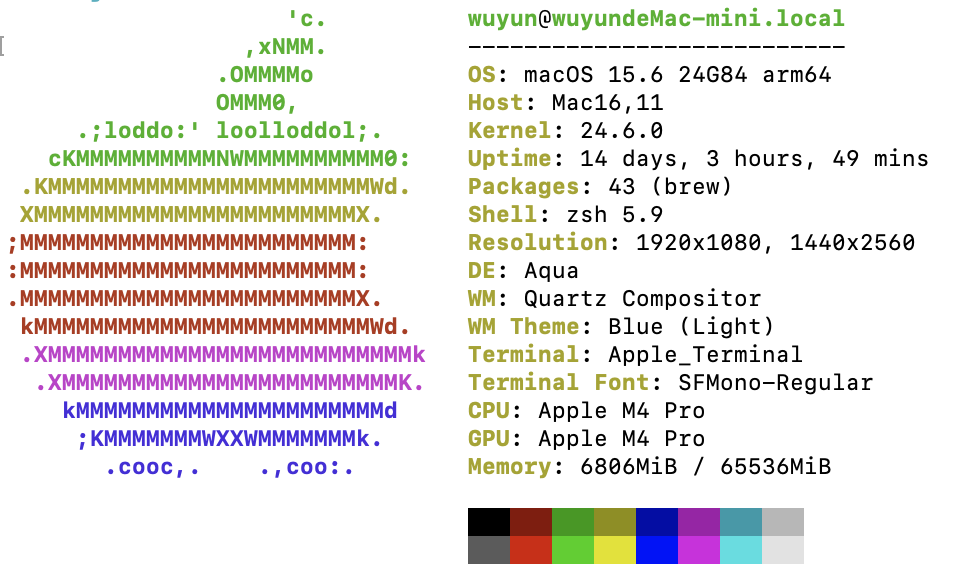
\includegraphics[width=0.85\linewidth]{macosconfig.png}
    \caption{System configuration used for halo2-lib and Midnight zk benchmarking.}
    \label{fig:system-config}
\end{figure}

\subsection{Benchmark Results}

We executed multi-scalar multiplication (MSM) benchmarks on both \texttt{halo2-lib} and Midnight zk. 
Table~\ref{tab:msm-comparison} extracts the key parameters---circuit size $k$, proving latency, proof size, and verification latency---to highlight the trade-offs across the two proving stacks.

\begin{table}[htbp]
    \centering
    \caption{MSM benchmarks.}
    \label{tab:msm-comparison}
    \begingroup
    \setlength{\tabcolsep}{4pt}
    \renewcommand{\arraystretch}{1.2}
    \begin{tabular}{ccccccc}
        \toprule
        \multirow{2}{*}{Concurrency} & \multicolumn{3}{c}{Midnight zk} & \multicolumn{3}{c}{halo2-lib} \\
        \cmidrule(lr){2-4} \cmidrule(lr){5-7}
         & \shortstack{Proof time\\(s)} & \shortstack{Proof size\\(bytes)} & \shortstack{Verify time\\(ms)} & \shortstack{Proof time\\(s)} & \shortstack{Proof size\\(bytes)} & \shortstack{Verify time\\(ms)} \\
        \midrule
        16 & 1.32 & 4\,864 & 3.06 & 12.48 & 1\,696 & 12.41 \\
        32 & 2.58 & 4\,864 & 3.20 & 13.61 & 1\,920 & 13.43 \\
        64 & 5.06 & 4\,864 & 3.12 & 26.78 & 1\,920 & 24.56 \\
        128 & 9.88 & 4\,864 & 3.20 & 86.23 & 1\,344 & 80.68 \\
        256 & 20.02 & 4\,864 & 3.42 & 56.39 & 4\,928 & 52.95 \\
        512 & 40.58 & 4\,864 & 3.14 & 135.88 & 2\,496 & 493.41 \\
        1\,024 & 83.84 & 4\,864 & 3.15 & 238.04 & 4\,704 & 524.87 \\
        \bottomrule
    \end{tabular}
    \endgroup
\end{table}


\end{document}
